\chapter{Experiments and Results}
\label{chap:results}

\section{Experimental Setup}
\label{sec:exp:setup}

\subsection{Parameter Ranges}
\label{sec:exp:params}

\TODO{Table of fixed and swept parameters: $N \in \{4, 6, 8, 10, 14, 18\}$,
budget $M_{\max}$, per-photon error rate, gate error rate, memory $T_2$.}

\subsection{Baselines}
\label{sec:exp:baselines}

\TODO{Define the baselines: (1)~raw chain, (2)~the paper's hand-chosen
YY-first fixed schedule (\texttt{flexible\_paper}), (3)~uniform
link-level purification with identical circuit sequence at every hop.}

\subsection{Metrics}
\label{sec:exp:metrics}

\TODO{Define the reported metrics: final Bell-pair fidelity $F$,
effective generation rate $R = P_{\mathrm{success}} / T_{\mathrm{gen}}$,
and resource consumption $M_{\mathrm{used}}$.}

\section{Validation}
\label{sec:exp:validation}

\TODO{Show that the DAG evaluator reproduces the three closed-form
timing/fidelity benchmarks from the Integrating paper for the canonical
schedule types. Include a table or figure comparing analytical and
simulated values.}

\section{Main Results}
\label{sec:exp:results}

\subsection{Schedule Structure at Optimal Points}
\label{sec:exp:optimal-structure}

\TODO{Present the dominant structural patterns discovered by the search
(e.g., YY-first at RGSS level, mixed ZX/XZ at link level). Use dot-graph
figures of representative optimal DAGs.}

\subsection{Throughput and Fidelity Comparison}
\label{sec:exp:comparison}

\begin{figure}[ht]
    \centering
    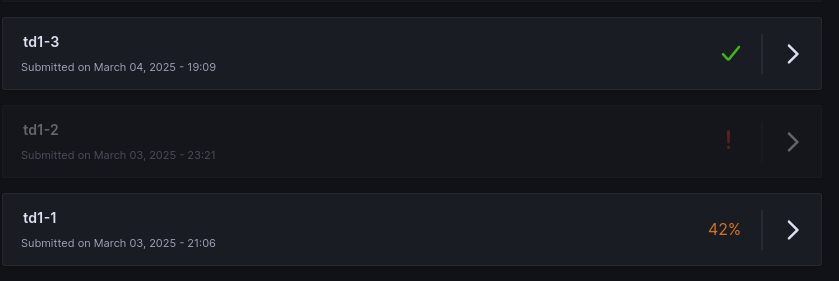
\includegraphics[width=.7\linewidth]{figures/results/throughput.png}
    \caption{\TODO{Effective rate vs.\ fidelity for competing scheduling
             strategies at $N=10$.}}
    \label{fig:throughput}
\end{figure}

\TODO{Discuss the Pareto frontier of (rate, fidelity) and where the
paper baseline and discovered optima sit on it.}

\subsection{Scaling with Hop Count}
\label{sec:exp:scaling}

\TODO{Show how the optimality gap between the baseline and the
discovered schedule evolves with $N$. Identify the crossover point.}

\subsection{Minimum Budget vs.\ Number of Hops}
\label{sec:exp:budget}

\TODO{Present the sweep over $(N, M_{\max})$ showing the minimum budget
needed to reach a target fidelity. Discuss the excluded-move gap.}